% Ubah judul dan label berikut sesuai dengan yang diinginkan.
\section{Desain dan Implementasi}
\label{sec:desaindanimplementasi}

\subsection{Deskripsi Sistem}
\label{subsec:deskripsisistem}

Pada tahap ini, kursi roda otonom dikembangkan untuk dapat mengikuti manusia menggunakan algoritma deteksi berbasis YOLOv11. Sistem ini dirancang dengan tujuan utama meningkatkan mobilitas pengguna yang membutuhkan bantuan dalam bergerak. Sistem terdiri dari komponen perangkat keras dan perangkat lunak, yang terintegrasi untuk mencapai tujuan ini.

\subsubsection{Komponen Sistem}
\label{subsubsec:komponensistem}

Sistem ini terdiri dari:

\begin{itemize}
    \item \textbf{VS Code}: Digunakan sebagai lingkungan pengembangan untuk menjalankan kode terkait YOLOv11 dan analisis lainnya.
    \item \textbf{Arduino IDE}: Mengembangkan dan mengunggah kode ke ESP32 yang mengendalikan motor dan sensor.
    \item \textbf{Laptop}: Berfungsi sebagai pusat pemrosesan data yang lebih kompleks dan pengembangan perangkat lunak.
    \item \textbf{Kamera (OV5640 5MP)}: Menangkap gambar lingkungan secara real-time dan mendeteksi target (manusia) menggunakan YOLOv11.
    \item \textbf{ESP32 Devkit V1}: Berfungsi sebagai pengontrol utama yang mengelola data dari kamera dan mengendalikan pergerakan kursi roda.
    \item \textbf{2 Kontroller Motor}: Mengendalikan motor DC yang menggerakkan kursi roda.
    \item \textbf{2 DC-DC Voltage Regulator}: Mengatur tegangan untuk komponen elektronik agar tetap stabil.
    \item \textbf{2 Motor DC}: Menggerakkan kursi roda, dikontrol melalui driver motor yang menerima sinyal dari mikroprosesor.
    \item \textbf{Baterai 24V}: Sebagai sumber daya utama untuk keseluruhan sistem, termasuk mikroprosesor, motor, dan perangkat lainnya.
\end{itemize}

\subsubsection{Arsitektur Sistem}
\label{subsubsec:arsitektursistem}

Arsitektur sistem dirancang agar kamera menangkap gambar secara terus-menerus, kemudian mengirimkan data ke mikroprosesor ESP32 untuk diproses. YOLOv11 digunakan untuk mendeteksi manusia dan memberikan informasi koordinat posisi target. Informasi ini kemudian digunakan oleh mikroprosesor untuk mengontrol motor dan mengarahkan kursi roda agar dapat mengikuti pergerakan target secara dinamis.

\subsection{Perangkat Keras}
\label{subsec:perangkathardware}

Desain perangkat keras melibatkan integrasi antara beberapa komponen yang disebutkan sebelumnya. Kamera dipasang di bagian depan kursi roda untuk mendapatkan sudut pandang optimal terhadap target. Mikroprosesor ESP32 ditempatkan di bagian bawah kursi roda bersama dengan driver motor dan baterai untuk menjaga keseimbangan.

\begin{itemize}
    \item \textbf{Unit Kontrol}: Unit Kontrol seperti komputer atau laptop digunakan sebagai pusat pemrosesan utama untuk menjalankan YOLOv11 dan mediapipe, menganalisis hasil deteksi dan menghasilkan keputusan berupa kode instruksi.
    \item \textbf{Kamera OV5640}: Kamera ini terhubung ke ESP32 untuk menangkap frame dengan menggunakan sensor 5MP.
    \item \textbf{ESP32}: Microcontroller ini menerima data dari kamera dan kemudian menjalankan algoritma untuk diproses pada komputer, lalu mengirim sinyal kontrol ke driver motor.
    \item \textbf{Driver Motor L298N}: Driver ini digunakan untuk mengontrol kecepatan dan arah putaran motor DC yang menggerakkan kursi roda.
\end{itemize}

\subsubsection{Kamera}
\label{subsubsec:kamera}
Kamera yang digunakan dalam sistem ini adalah OV5640, sebuah sensor kamera CMOS (Complementary Metal-Oxide-Semiconductor) dengan resolusi 5 megapiksel (MP). Sensor ini memiliki kemampuan menangkap gambar hingga resolusi maksimum 2592x1944 piksel, yang memberikan hasil citra dengan detail yang sangat baik. Sensor ini mendukung pengambilan gambar dan video secara real-time, dengan frame rate mencapai 30 frame per detik (fps) pada resolusi 1080p, sehingga ideal untuk aplikasi yang memerlukan pengolahan citra secara langsung.

Selain resolusinya yang tinggi, OV5640 juga dilengkapi dengan berbagai fitur canggih untuk pengolahan gambar otomatis. Berdasarkan datasheet, fitur seperti auto white balance, auto exposure, dan auto focus memungkinkan kamera ini beradaptasi secara otomatis terhadap perubahan kondisi pencahayaan dan jarak, sehingga tetap menghasilkan gambar berkualitas tinggi dalam berbagai situasi. OV5640 juga mendukung fitur face detection dan image scaling, yang sangat berguna dalam mendeteksi objek atau target manusia secara cepat dan akurat.

\subsubsection{Unit Kontrol}
\label{subsubsec:UnitKontrol}
% Pada sistem ini, unit kontrol utama yang digunakan adalah laptop pribadi yang berperan sebagai pengolah data utama selama pengujian. Laptop ini memiliki spesifikasi yang dirancang untuk menangani beban komputasi tinggi, sangat cocok untuk pengolahan data secara real-time, sebagaimana ditunjukkan pada tabel.

% \begin{table}[H]
%   \centering
%   \caption{Spesifikasi Laptop MSI GF63 untuk Unit Kontrol}
%   \begin{tabular}{|l|l|}
%   \hline
%   \textbf{Komponen}       & \textbf{Spesifikasi}                     \\ \hline
%   Model Laptop            & MSI GF63                                 \\ \hline
%   Prosesor                & Intel Core i7-10750H, 6 core, 12 threads \\ \hline
%   GPU                     & NVIDIA RTX 3050                          \\ \hline
%   RAM                     & 16GB DDR4, 3200 MHz                      \\ \hline
%   Penyimpanan             & SSD M.2                                  \\ \hline
%   Konektivitas WiFi       & WiFi 802.11ac (MU-MIMO)                  \\ \hline
%   Pengolahan Data         & Inferensi model, ESP dan Python (venv)   \\ \hline
%   \end{tabular}
% \end{table}

Unit kontrol pada sistem ini, berperan sebagai pengolah data utama selama pengujian, dengan spesifikasi yang dirancang untuk menangani beban komputasi tinggi dan cocok untuk pengolahan data secara real-time.

Salah satu aspek penting dari unit kontrol dalam proyek ini adalah dukungan WiFi yang cepat dan stabil dalam komunikasi antar perangkat. Sistem bergantung pada data video yang dikirim oleh kamera OV5640 melalui ESP32 ke laptop untuk diolah, dan proses ini harus berlangsung tanpa hambatan. Konektivitas WiFi yang disediakan juga memungkinkan pengiriman data dalam waktu nyata dengan minim latensi, yang sangat penting untuk deteksi target secara cepat.

Kemampuan untuk menjaga kestabilan koneksi WiFi pada jarak yang lebih jauh dari router juga penting dalam pengujian di area yang luas. Seperti dengan menangani beberapa perangkat yang terhubung secara simultan, memungkinkan komunikasi yang efisien antara ESP32 tanpa penurunan performa. Teknologi ini sangat penting untuk memastikan bahwa sistem dapat terus memproses data video yang dikirimkan oleh kamera dan memberikan instruksi dengan respons yang cepat.

Data citra yang didapatkan menggunakan kamera OV5640, selanjutnya akan diproses melalui serangkaian pengolahan data citra menggunakan model deteksi yang telah dilatih sebelumnya. Model ini dilatih menggunakan arsitektur YOLOv11. Model yang digunakan diberi nama Best.pt, yang merupakan file hasil pelatihan yang telah di \emph{training} untuk mendeteksi kelas Manusia.

Agar sistem dapat diimplementasikan dengan baik, beberapa library atau pustaka perlu diinstal terlebih dahulu. Library tersebut mencakup OpenCV untuk pengolahan citra, Ultralytics untuk Yolo.

\begin{lstlisting}
  pip install OpenCV
  pip install Ultralytics
  ...dll
\end{lstlisting}

\subsubsection{ESP32}
\label{subsubsec:ESP32}
ESP32 akan menerima data arah dari hasil klasifikasi deteksi manusia dalam bentuk karakter huruf seperti A, B, C, D, atau E. Berdasarkan penelitian sebelumnya, proses penerimaan data string oleh ESP32 dari perangkat yang terhubung sangat penting untuk kelancaran sistem.

Setelah data diterima dan disimpan, string tersebut diekstrak menjadi informasi tentang arah dan kecepatan. Tahap ekstraksi ini krusial untuk mengubah string menjadi format yang dapat digunakan oleh program dalam mengendalikan motor kursi roda. Data yang telah diekstrak kemudian ditampilkan untuk memastikan bahwa arah dan kecepatan yang diterima sesuai dengan yang diharapkan. Dengan informasi arah dan kecepatan yang sudah siap, ESP32 dapat mengirimkan instruksi ke motor kursi roda agar bergerak sesuai dengan data yang diterima. Proses ini akan terus berulang selama perangkat tetap terhubung dan data terus mengalir.

Untuk memberikan pemahaman yang lebih jelas mengenai instruksi yang diterima dari hasil klasifikasi deteksi manusia, berikut disajikan kode instruksi yang digunakan dalam program ini:
\begin{table}[H]
\centering
\caption{Kode Instruksi dari Hasil Klasifikasi}
\begin{tabular}{|c|c|}
\hline
\textbf{Klasifikasi Pose} & \textbf{Kode Instruksi} \\
\hline
Kiri & A \\
\hline
Maju & B \\
\hline
Stop & C \\
\hline
Mundur & D \\
\hline
Kanan & E \\
\hline
\end{tabular}
\end{table}

Kode instruksi tersebut digunakan untuk mengarahkan motor kursi roda sesuai dengan deteksi yang dilakukan oleh model klasifikasi YOLOv11. Misalnya, jika arah yang terdeteksi adalah "Kiri", maka kode instruksi 'A' akan dikirim untuk menggerakkan kursi roda ke kiri. Demikian pula, jika terdeteksi arah "Maju", instruksi 'B' akan dikirim untuk menggerakkan kursi roda maju. Kode 'C' digunakan untuk menghentikan kursi roda saat terdeteksi "Stop", 'D' untuk bergerak mundur ketika terdeteksi "Mundur", dan 'E' untuk bergerak ke kanan saat terdeteksi "Kanan".

Program ini memastikan bahwa ESP32 berfungsi secara efektif sebagai server yang menerima data dari NUC dan menggunakannya untuk mengendalikan motor kursi roda. Dengan langkah-langkah yang telah dijelaskan, program ini dirancang untuk berjalan secara kontinu tanpa henti, menunggu dan memproses data yang dikirim oleh perangkat yang terhubung.

\subsubsection{Driver Motor L298N}
\label{subsubsec:drivermotor}
Driver motor yang digunakan dalam sistem ini adalah L298N, yang berperan penting dalam pengendalian motor DC pada kursi roda. Driver ini berfungsi sebagai perantara antara mikrokontroler dan motor, dengan menerima sinyal kontrol dari ESP32 dan meneruskannya ke motor. Penggunaan driver L298N memungkinkan sinyal digital diubah menjadi sinyal yang dapat diterima oleh motor, sehingga motor dapat beroperasi sesuai dengan instruksi yang diberikan.

Driver L298N mampu mengendalikan dua motor DC secara simultan dengan fitur pengaturan kecepatan dan arah putaran motor. Driver ini bekerja dengan prinsip rangkaian H-Bridge, yang memungkinkan perubahan arah arus untuk mengatur rotasi motor maju atau mundur. Selain itu, L298N dilengkapi dengan fitur pengaturan kecepatan melalui teknik Pulse Width Modulation (PWM), yang memberikan kendali yang lebih akurat terhadap kecepatan motor. Dengan fitur ini, kursi roda dapat bergerak maju, mundur, berbelok, atau berhenti sesuai instruksi yang diterima.

\subsubsection{Skematik Alat}
\label{subsubsec:skematikalat}

Dari penelitian yang telah dilakukan, telah dirancang sebuah sistem kontrol untuk motor kursi roda dengan skematik alat yang ditampilkan pada Gambar \ref{fig:Skematik Kontrol motor Kursi roda.}. ESP32 akan terhubung dengan dua buah H-Bridge Motor Driver dan sebuah DC-DC Converter. Setiap H-Bridge Motor Driver terhubung langsung ke motor roda kiri dan motor roda kanan untuk menggerakkan roda kursi roda secara efektif. Dalam skematik ini, ESP32 berfungsi sebagai otak dari sistem, mengirimkan sinyal kontrol ke motor driver berdasarkan data yang diterima melalui koneksi WiFi. \cite{ekatama2024perancangan}

Dalam penelitian ini, digunakan dua metode kontrol untuk menggerakkan kursi roda. Metode pertama adalah differential drive, ketika kursi roda berbelok ke kanan, roda kanan akan bergerak mundur dan berbelok ke kiri, sedangkan roda kiri bergerak maju dan berbelok ke kanan. Sebaliknya, ketika berbelok ke kiri, roda kiri akan bergerak mundur dan berbelok ke kanan, sedangkan roda kanan bergerak maju dan berbelok ke kiri. Metode kedua adalah pergerakan biasa, ketika kursi roda berbelok ke kanan, roda kanan akan diam sedangkan roda kiri bergerak maju dan berbelok ke kanan, dan sebaliknya untuk berbelok ke kiri. Saat bergerak maju atau mundur, kedua roda bergerak secara bersamaan ke arah yang diinginkan. Untuk penelitian kali ini, metode kedua digunakan untuk menggerakkan roda pada kursi roda.

Dengan demikian, program ini memastikan bahwa ESP32 dapat berfungsi secara efektif sebagai pengontrol motor kursi roda. Setiap langkah dalam flowchart dirancang untuk memastikan bahwa sistem dapat berjalan secara efisien dan responsif terhadap perintah yang diterima melalui jaringan WiFi. Sistem ini dirancang untuk beroperasi secara real-time, memberikan respon cepat terhadap perubahan perintah, dan mengendalikan kursi roda secara akurat berdasarkan data yang diterima.

Skematik yang ditampilkan memberikan gambaran yang jelas mengenai alur kerja dan koneksi perangkat keras yang digunakan dalam sistem kontrol ini. Dengan penjelasan yang mendetail, setiap aspek dari sistem ini dapat dipahami dengan baik, memastikan implementasi yang tepat dan operasi yang efisien dari kursi roda yang dikendalikan secara otonom. \cite{ekatama2024perancangan}

\begin{figure}[H]
  \centering

  % Ubah dengan nama file gambar dan ukuran yang akan digunakan
  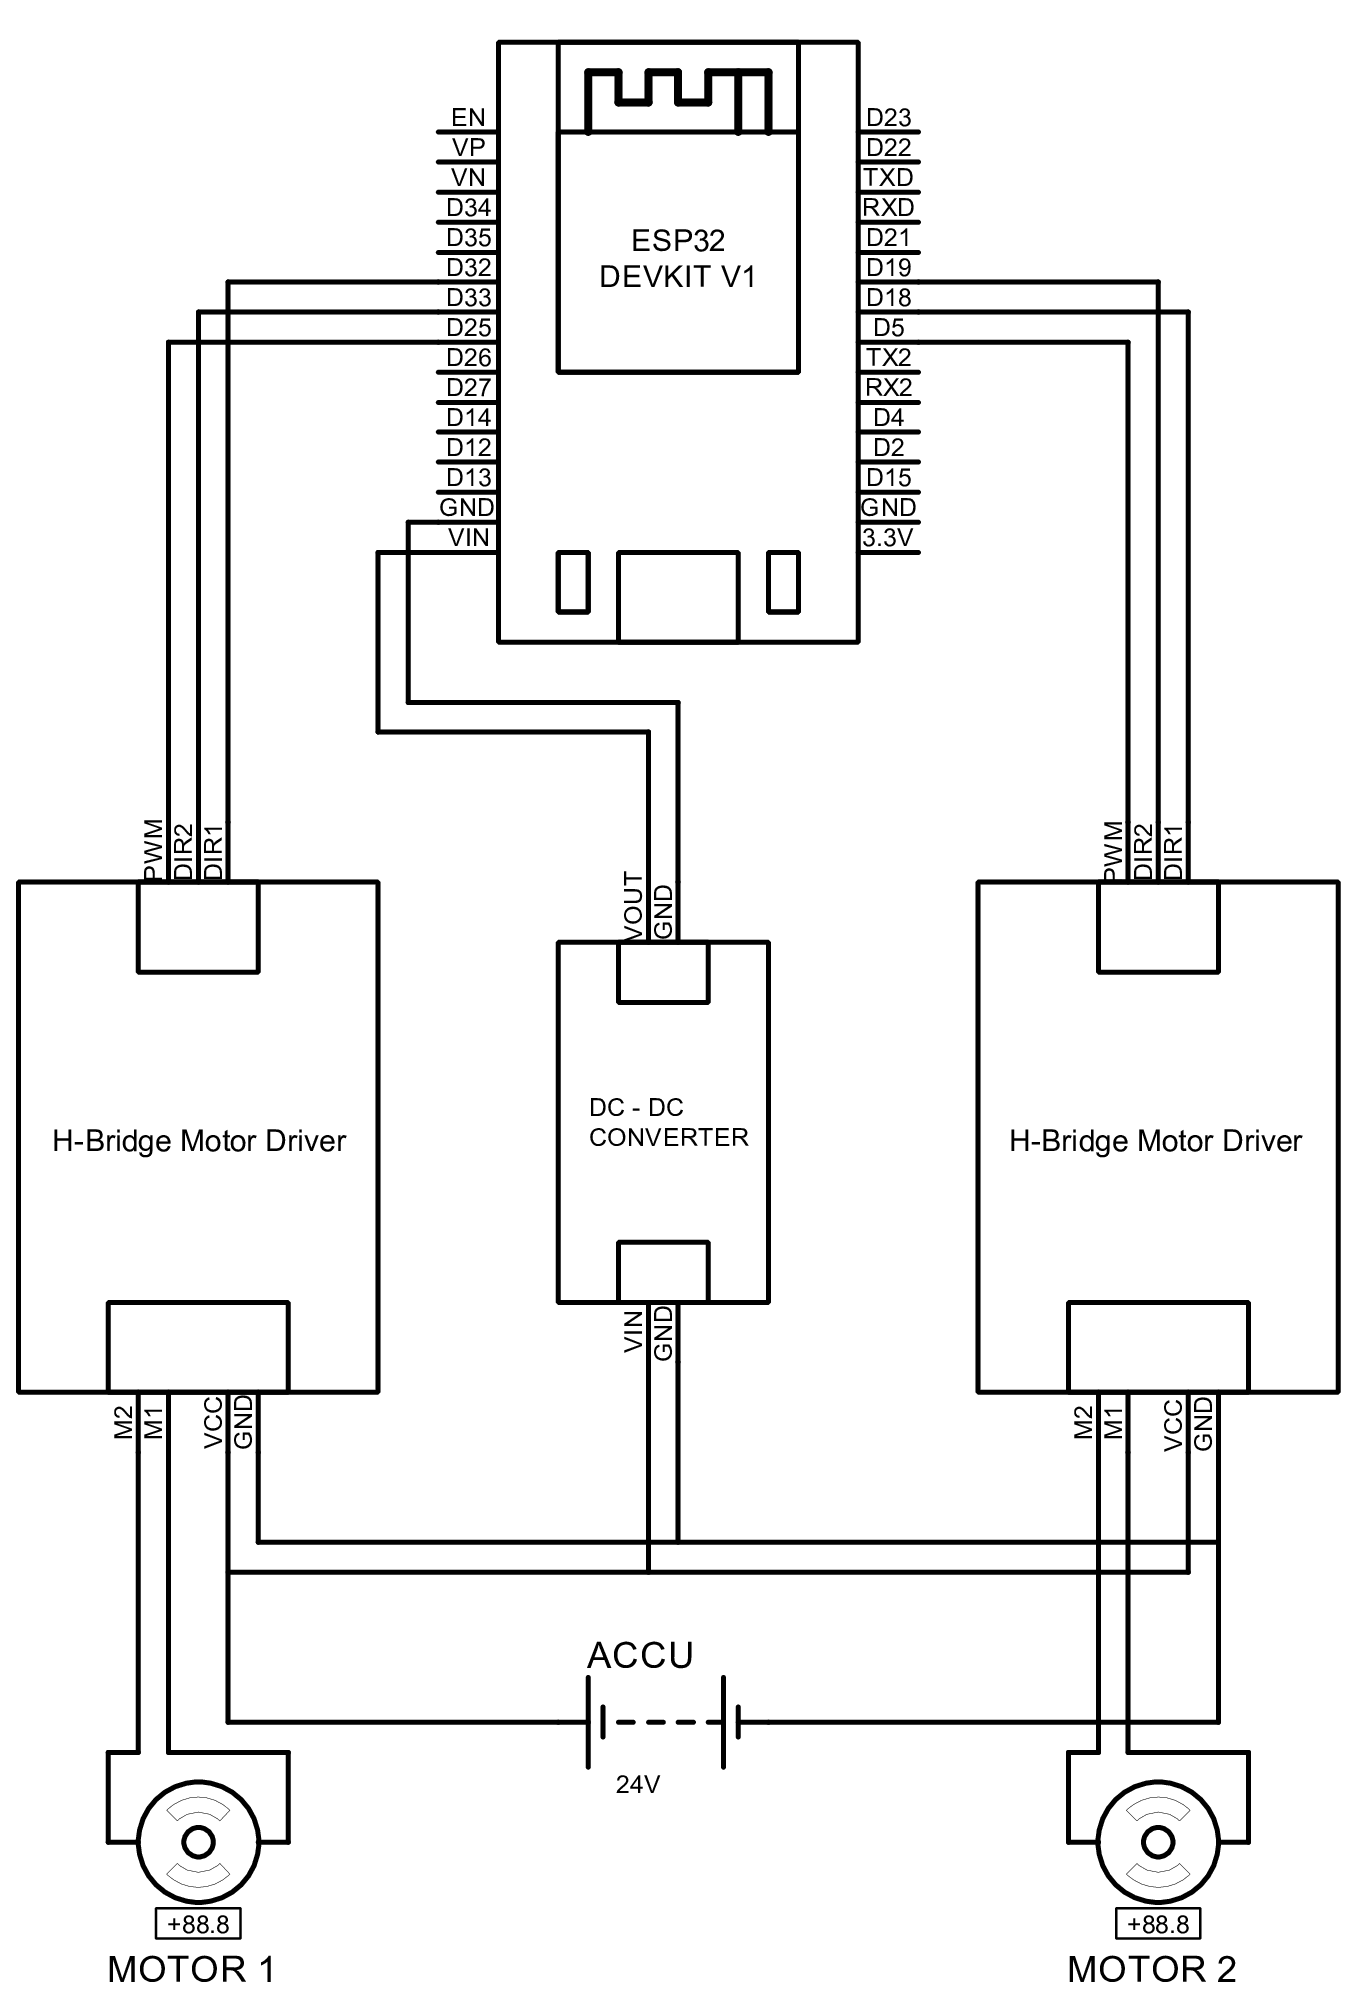
\includegraphics[scale=0.2]{gambar/Schematics.png}

  % Ubah dengan keterangan gambar yang diinginkan
  \caption{Skematik kontrol motor kursi roda}
  \label{fig:Skematik Kontrol motor Kursi roda.}
\end{figure}

\subsection{Perangkat Lunak}
\label{subsec:perangkatlunak}

Perangkat lunak yang digunakan dalam sistem ini terdiri dari beberapa modul, yang meliputi:

\begin{itemize}
    \item \textbf{Algoritma Deteksi YOLOv11}: YOLOv11 digunakan untuk mendeteksi manusia dalam gambar yang ditangkap oleh kamera. Model ini dilatih untuk mengenali bentuk dan posisi manusia sehingga kursi roda dapat mengikuti target dengan tepat.
    \item \textbf{Estimasi Pose MediaPipe}: MediaPipe digunakan untuk mendeteksi landmark tubuh manusia setelah objek terkunci. Framework ini dipilih karena kemampuannya dalam mendeteksi keypoints pada tubuh manusia dengan akurasi tinggi, bahkan dalam kondisi pencahayaan yang beragam.
    \item \textbf{Komunikasi Data}: Sistem menggunakan protokol MQTT untuk mengirimkan data antara ESP32 yang terhubung ke kamera dan unit kontrol utama.
    \item \textbf{Kontrol Motor}: Modul kontrol motor diimplementasikan pada ESP32 untuk mengatur arah dan kecepatan motor berdasarkan posisi target yang terdeteksi.
\end{itemize}

\subsubsection{Dataset Citra}
\label{subsubsec:datasetcitra}

Dataset citra yang digunakan dalam penelitian ini terdiri dari kumpulan gambar yang diambil menggunakan kamera OV5640. Objek yang dideteksi pada gambar ini adalah manusia, yang difungsikan sebagai target untuk diikuti oleh kursi roda. Dataset mencakup berbagai pose dan posisi manusia, serta kondisi pencahayaan yang berbeda, agar model YOLOv11 dapat dilatih secara optimal dalam mengenali target dalam berbagai situasi. Gambar-gambar ini diperoleh dari setiap frame video yang diambil menggunakan kamera yang terhubung dengan komputer. Proses pendeteksian dilakukan secara real-time untuk memastikan sistem mampu mengidentifikasi target secara berkelanjutan.

\subsubsection{Labeling}
\label{subsubsec:labeling}

Dataset citra yang telah diperoleh kemudian melalui proses labeling dan augmentasi menggunakan alat seperti Roboflow, yang menyediakan berbagai fitur untuk mempermudah proses ini. Proses labeling ini melibatkan impor dataset, pemberian label pada setiap gambar, dan augmentasi data. Labeling dilakukan untuk memastikan bahwa setiap objek dalam gambar dikenali dengan benar, terutama manusia yang menjadi target. Penamaan class harus konsisten dengan objek yang akan dideteksi untuk memastikan model YOLOv11 dapat dilatih dengan baik.

Selain itu, Roboflow juga menyediakan fitur preprocessing dataset yang membantu menstandarkan format gambar, misalnya mengubah ukuran semua gambar menjadi seragam. Langkah ini penting untuk menjaga konsistensi dataset sebelum melatih model. Beberapa fitur yang tersedia antara lain Auto-Orient, Resize, Grayscale, Auto Adjust Contrast, Isolate Objects, Static Crop, Tile, Modify Classes, dan Filter Null. Preprocessing ini memastikan bahwa data yang digunakan memiliki kualitas yang seragam untuk meningkatkan performa model.

Fitur augmentasi data juga disediakan untuk menambah variasi pada dataset. Augmentasi bertujuan untuk meningkatkan keragaman dalam dataset, yang pada akhirnya membantu meningkatkan performa model dalam mendeteksi manusia. Proses augmentasi ini sangat penting dalam tugas akhir ini karena membutuhkan variasi yang luas dalam data citra manusia, yang memungkinkan sistem lebih robust dalam berbagai kondisi.

\subsubsection{Klasifikasi YOLOv11}
\label{subsubsec:klasifikasiYOLOv11}

Dalam proses klasifikasi, setiap citra yang telah melalui proses labeling dikenali dengan menggunakan YOLOv11 yang telah dilatih untuk mendeteksi manusia pada citra. Model ini mampu mendeteksi keberadaan manusia secara akurat dan real-time, memungkinkan sistem untuk mengidentifikasi target dengan efisien. Setiap citra diproses oleh model YOLOv11, yang kemudian memberikan output berupa bounding box dan confidence score yang menunjukkan keberadaan manusia serta keyakinan model terhadap deteksi tersebut. Proses ini dilakukan secara real-time, memungkinkan sistem untuk memberikan umpan balik langsung ke kontrol kursi roda berdasarkan deteksi manusia dalam gambar.

Model YOLOv11 yang digunakan memiliki output kelas utama yaitu manusia. Model ini menghasilkan bounding box, yang menunjukkan area lokasi objek, dan confidence score untuk memberikan keyakinan deteksi. Algoritma YOLOv11 menggunakan Convolutional Neural Network (CNN) sebagai basisnya, yang berfungsi untuk mengekstraksi fitur dari gambar input, lalu memprediksi bounding box dan kelas objek langsung dari gambar tersebut. Proses ini diilustrasikan pada Gambar, yang menunjukkan blok diagram arsitektur model YOLOv11.

YOLOv11 terdiri dari beberapa lapisan, antara lain Conv2D (Convolutional 2D), Blok C2f, Blok SPPF (Spatial Pyramid Pooling Fast), lapisan Upsampling, dan lapisan Concatenate. Setiap lapisan ini memiliki peran tertentu dalam memproses gambar, mengekstraksi fitur, dan membuat prediksi yang tepat. Lapisan Conv2D digunakan untuk mengekstraksi fitur dari gambar input, sementara Blok C2f dan SPPF membantu dalam pemrosesan informasi dari berbagai skala untuk menangkap detail yang lebih baik. Lapisan Upsampling digunakan untuk meningkatkan resolusi fitur, sementara lapisan Concatenate menggabungkan berbagai informasi dari jalur yang berbeda untuk membuat representasi yang lebih kuat.

Gambar menunjukkan setiap jenis lapisan dalam YOLOv11 dengan warna yang berbeda, seperti lapisan Conv2D yang ditampilkan dalam warna biru, Blok C2f dengan warna kuning, lapisan SPPF dengan warna hijau muda, lapisan Upsampling dengan warna merah muda, dan lapisan Concatenate dengan warna ungu. Visualisasi ini membantu memahami bagaimana model YOLOv11 memproses gambar dan bagaimana setiap lapisan berkontribusi dalam menghasilkan bounding box dan prediksi kelas yang akurat. Selain itu, input dan output dari setiap lapisan dapat dilihat pada Gambar, yang menggambarkan detail dari tiap proses pemrosesan dalam model YOLOv11.

Lapisan deteksi pada YOLOv11 menghasilkan output yang mencakup bounding box dan confidence score untuk manusia yang terdeteksi, yang kemudian digunakan sebagai acuan dalam sistem untuk mengikuti target. Model ini dioptimalkan untuk dapat mengenali manusia dengan berbagai posisi dan kondisi pencahayaan, sehingga kursi roda dapat beradaptasi dengan pergerakan target dalam berbagai situasi secara efektif.

\subsubsection{Estimasi Pose MediaPipe}
\label{subsubsec:estimasi_pose_mediapipe}

Pada penelitian ini, pose manusia dideteksi menggunakan Python dengan library OpenCV dan MediaPipe. Proses dimulai setelah objek manusia terdeteksi dalam frame, di mana MediaPipe kemudian digunakan untuk mengidentifikasi landmark pada tubuh. MediaPipe dipilih karena kemampuannya mendeteksi titik kunci (keypoints) pada tubuh manusia dengan akurasi tinggi dalam berbagai kondisi pencahayaan dan posisi. Setelah landmark berhasil dideteksi, titik-titik yang relevan akan digambarkan menggunakan garis untuk membentuk kerangka sesuai dengan pose tubuh.

Proses deteksi diawali dengan inisialisasi kamera yang menangkap frame secara real-time. Setelah frame diterima, dilakukan pra-pengolahan seperti konversi gambar ke skala abu-abu untuk mengurangi kompleksitas dan meningkatkan kecepatan deteksi. Gambar yang telah dipra-pengolah tersebut kemudian diproses oleh model MediaPipe untuk mendeteksi pose.

Dalam penelitian ini, beberapa landmark yang dipilih untuk analisis adalah titik-titik pada siku, lengan bawah, dan bahu kanan serta kiri. Pemilihan titik-titik ini didasarkan pada visibilitas dan konsistensi dalam proses deteksi. Tabel menampilkan nomor dan nama keypoint yang digunakan dalam estimasi pose:

\begin{table}[H]
  \centering
  \caption{Tabel Keypoint yang digunakan}
  \label{tab:keypoints}
  \begin{tabular}{|c|c|}
    \hline
    Nomor Keypoint & Nama Keypoint \\
    \hline
    11 & RIGHT SHOULDER \\
    12 & LEFT SHOULDER \\
    14 & RIGHT ELBOW \\
    16 & RIGHT WRIST \\
    \hline
  \end{tabular}
\end{table}

Setelah landmark diperoleh, jarak antar titik pada piksel dihitung. Pengukuran ini dilakukan dengan menggunakan jarak Euclidean antara dua titik kunci, yang merupakan metode efisien untuk menghitung jarak dalam ruang dua dimensi. Nilai jarak ini kemudian digunakan sebagai acuan untuk pergerakan kursi roda mengikuti target di depan.

\subsubsection{Pemrosesan Citra}
\label{subsubsec:pemrosesan_citra}

Pemrosesan citra dilakukan untuk meningkatkan kualitas gambar yang diambil dari kamera dan mempermudah deteksi objek. Langkah-langkah pemrosesan citra meliputi konversi warna, penghilangan noise, dan pemfilteran tepi untuk menyorot bagian-bagian penting dari gambar.

\subsubsection*{Pembuatan Tracking ID untuk Mengunci Target}
\label{subsubsec:tracking_id}

Sistem ini memanfaatkan Ultralytics YOLO untuk mendeteksi target manusia dalam setiap frame, lalu memberikan ID unik pada setiap objek yang terdeteksi. ID tersebut berfungsi untuk mengidentifikasi dan melacak individu yang sama pada frame berikutnya, memungkinkan untuk terus mengikuti target meskipun terjadi pergerakan dalam frame. Deteksi yang akurat dan pemberian ID ini sangat penting agar kursi roda dapat merespons secara tepat terhadap perubahan posisi target.

\subsubsection*{Keputusan untuk Bergerak Maju}
\label{subsubsec:keputusan_bergerak_maju}

Setelah target terdeteksi dan tracking ID dibuat, sistem akan menghitung jarak antara kursi roda dengan target. Jika jarak target berada dalam kisaran yang aman dan berada di tengah frame, sistem akan mengirimkan perintah untuk bergerak maju. Hal ini dilakukan dengan menggunakan algoritma yang menghitung jarak dari bounding box target dan memastikan bahwa target berada pada posisi yang tepat untuk diikuti.

\subsubsection*{Keputusan untuk Berbelok ke Kiri}
\label{subsubsec:keputusan_belok_kiri}

Jika target bergerak ke arah kiri dan keluar dari batas tengah frame, kursi roda akan mengirimkan perintah untuk berbelok ke kiri. Sistem mendeteksi posisi target di bagian kiri frame dan memberikan instruksi ke motor untuk mengarahkan kursi roda ke kiri agar tetap dapat mengikuti pergerakan target secara optimal.

\subsubsection*{Keputusan untuk Berbelok ke Kanan}
\label{subsubsec:keputusan_belok_kanan}

Sebaliknya, jika target bergerak ke arah kanan dan keluar dari batas tengah frame, sistem akan mengirimkan perintah untuk berbelok ke kanan. Posisi target yang berada di sisi kanan frame akan memicu motor untuk berbelok ke kanan, memastikan kursi roda dapat menyesuaikan posisinya dengan target yang bergerak.

\subsubsection*{Keputusan Jika Target Menghilang dari Frame}
\label{subsubsec:keputusan_target_menghilang}

Apabila target menghilang dari frame, sistem akan mencari target berdasarkan posisi terakhir yang terdeteksi. Jika ada target baru yang terdeteksi di frame, sistem akan membuat tracking ID baru dan melanjutkan pelacakan terhadap target tersebut. Sistem akan menunggu hingga target muncul kembali dalam frame atau mendeteksi target baru untuk melanjutkan pelacakan. Pendekatan ini memastikan bahwa kursi roda bergerak sesuai arah terakhir ketika target tidak terlihat.

\subsubsection{Komunikasi Data}
\label{subsubsec:komunikasi_data}

Pada sistem ini, komunikasi data dilakukan menggunakan kombinasi WiFi dan ESP-NOW. WiFi digunakan untuk membangun Access Point pada ESP32 yang terhubung dengan kamera, memungkinkan streaming video real-time ke unit kontrol melalui jaringan lokal. Stream ini dapat diakses melalui server HTTP di port 81, di mana data video dari kamera diproses oleh unit kontrol untuk deteksi target.

Selain itu, ESP-NOW digunakan untuk pengiriman data secara langsung antara dua perangkat ESP32. Data yang diterima dari port 80 oleh ESP32 yang terhubung dengan kamera dikirimkan ke ESP32 lainnya (yang mengendalikan motor) melalui ESP-NOW. Protokol ini memungkinkan pertukaran data dengan latensi rendah tanpa memerlukan koneksi internet atau router eksternal. Dengan kombinasi ini, sistem dapat mempertahankan komunikasi yang cepat dan stabil, memastikan kursi roda dapat merespons pergerakan target secara real-time.

\subsubsection{Kontrol Motor}
\label{subsubsec:kontrol_motor}

Kontrol motor pada sistem kursi roda ini diimplementasikan menggunakan ESP32 yang bertindak sebagai pengendali utama untuk arah dan kecepatan motor. Setelah target manusia terdeteksi oleh kamera dan diproses oleh YOLOv11, informasi mengenai posisi target dikirim ke ESP32 untuk menentukan perintah pergerakan yang sesuai. Berdasarkan posisi target di dalam frame, ESP32 akan memberikan sinyal kepada driver motor untuk mengendalikan arah gerakan kursi roda, baik bergerak maju, berbelok ke kiri, berbelok ke kanan, atau berhenti.

Motor dikendalikan melalui sinyal PWM (Pulse Width Modulation) yang dihasilkan oleh ESP32, yang digunakan untuk mengatur kecepatan motor secara halus. Kombinasi sinyal arah dan PWM memungkinkan sistem untuk menggerakkan motor dengan responsif, baik untuk mengejar target, berbelok, atau berhenti secara tiba-tiba jika diperlukan. Selain itu, sistem juga menggunakan kontrol loop untuk terus memantau posisi target dan menyesuaikan pergerakan kursi roda secara real-time agar tetap dapat mengikuti target dengan akurat. Proses kontrol ini berlangsung terus-menerus untuk memastikan bahwa kursi roda selalu dapat beradaptasi dengan pergerakan target.

\subsubsection{Kode Program}
\label{subsubsec:kode_program}

Kode program yang digunakan dalam penelitian ini dimulai dengan inisialisasi variabel dan perangkat keras yang diperlukan, termasuk mengaktifkan kamera untuk menangkap gambar secara real-time. Setelah gambar diperoleh, algoritma YOLOv11 digunakan untuk mendeteksi keberadaan manusia dalam frame tersebut. Jika manusia terdeteksi, program melanjutkan dengan mengidentifikasi bounding box dan memberi label pada objek, yang kemudian digunakan untuk melacak objek tersebut di frame berikutnya. Setelah itu, framework MediaPipe diimplementasikan untuk mendeteksi landmark tubuh, seperti bahu, siku, dan pergelangan tangan, yang memungkinkan sistem memperoleh pose manusia secara lebih rinci.

\begin{figure}[H]
  \centering
  \resizebox{1\linewidth}{!}{
    \begin{tikzpicture}[node distance=2cm]
\node (start) [startstop] {Mulai};
\node (initVars) [process, below of=start] {Inisialisasi Variabel dan Hardware};
\node (captureFrame) [io, below of=initVars] {Ambil Frame dari Kamera};
\node (yoloDetect) [process, below of=captureFrame] {Deteksi Objek Menggunakan Yolo};
\node (A) [connector, below of=yoloDetect] {A};
\node (C0) [connector, left of=initVars, xshift=-1.5cm, yshift=-1cm] {C};

\node (A0) [connector, right of=start, xshift=4.5cm] {A};
\node (checkBoxes) [decision, below of=A0] {Deteksi Objek?};
\node (processBox) [process, below of=checkBoxes] {Proses Bounding Box};
\node (trackingID) [process, below of=processBox] {Proses Tracking ID};
\node (mediapipeProcessing) [process, below of=trackingID] {Deteksi Landmark Pose pada MediaPipe};
\node (B) [connector, below of=mediapipeProcessing, xshift=1.5cm] {B};

\node (B0) [connector, right of=A0, xshift=3.5cm] {B};
\node (calcDirection) [process, below of=B0] {Proses Kalkulasi Arah dan Jarak};
\node (controlWheelchair) [io, below of=calcDirection] {Kirim Data ke Kursi Roda};
\node (display) [io, below of=controlWheelchair] {Gambar Arah pada Frame};
\node (endLoop) [decision, below of=display, yshift=-.5cm] {Tombol 'q' Ditekan?};
\node (C) [connector, right of=endLoop, xshift=1cm, yshift=-1.5cm] {C};
\node (end) [startstop, below of=endLoop, yshift=-1cm] {Selesai};

\node (searchPerson) [process, below of=mediapipeProcessing, xshift=-3cm] {Memuat Arah dan Jarak Sebelumnya};

\draw [arrow] (start) -- (initVars);
\draw [arrow] (initVars) -- (captureFrame);
\draw [arrow] (captureFrame) -- (yoloDetect);
\draw [arrow] (yoloDetect) -- (A);
\draw [arrow] (C0) |- (captureFrame);

\draw [arrow] (A0) -- (checkBoxes);
\draw [arrow] (checkBoxes) -- node[anchor=west] {Ya} (processBox);
\draw [arrow] (processBox) -- (trackingID);
\draw [arrow] (trackingID) -- (mediapipeProcessing);
\draw [arrow] (mediapipeProcessing) -- +(0,-2cm);

\draw [arrow] (B0) -- (calcDirection);
\draw [arrow] (calcDirection) -- (controlWheelchair);
\draw [arrow] (controlWheelchair) -- (display);
\draw [arrow] (display) -- (endLoop);
\draw [arrow] (endLoop) -| node[anchor=south east] {Tidak} (C);
\draw [arrow] (endLoop) -- node[anchor=west] {Ya} (end);

\draw [arrow] (checkBoxes) -| node[anchor=south west] {Tidak} (searchPerson);
\draw [arrow] (searchPerson) -- (B);
\end{tikzpicture}
  }
  \caption{Flowchart program python}
\end{figure}

Program kemudian menghitung arah dan jarak target, yang digunakan untuk menentukan instruksi pergerakan kursi roda. Instruksi tersebut dikirimkan ke ESP32, yang mengendalikan motor kursi roda untuk mengikuti manusia secara otomatis. Selain itu, arah pergerakan digambarkan pada frame video yang ditampilkan sebagai bentuk visualisasi dari proses yang sedang berjalan. Program akan terus melakukan loop, menangkap gambar baru, memproses deteksi, dan mengirimkan perintah hingga pengguna menekan tombol 'q' untuk mengakhiri program.


\begin{figure}[H]
  \centering
  \resizebox{.7\linewidth}{!}{
    \begin{tikzpicture}[node distance=2cm]
\node (start) [startstop] {Mulai};
\node (getCurrentTime) [io, below of=start] {Ambil Waktu\\Saat ini};
\node (check_delay) [decision, below of=getCurrentTime, text width=2.5cm] {\emph{delay} \(\lor\) Data: C?};
\node (check_sent) [decision, below of=check_delay, yshift=-.5cm] {Sudah dikirim?};
\node (A) [connector, left of=check_sent, xshift=-1cm] {A};
\node (send_data) [process, below of=check_sent] {Mengirim data};
\node (sent_true) [process, below of=send_data] {Penanda data sudah dikirim};

\node (A0) [connector, right of=start, xshift=4cm, yshift=-.5cm] {A};
\node (check_update) [decision, below of=A0] {Data berubah?};
\node (send_C) [process, below of=check_update] {Mengirim 'C\textbackslash n'};
\node (check_input) [decision, below of=send_C] {Input: C?};
\node (update_data) [io, below of=check_input, text width=2.7cm] {Data diperbarui};
\node (sent_false) [process, below of=update_data] {Penanda data belum dikirim};
\node (stop) [startstop, below of=sent_false, xshift=-3cm] {Selesai};

\draw [arrow] (start) -- (getCurrentTime);
\draw [arrow] (getCurrentTime) -- (check_delay);
\draw [arrow] (check_delay) -- node[anchor=west] {Tidak} (check_sent);
\draw [arrow] (check_sent) -- node[anchor=west] {Tidak} (send_data);
\draw [arrow] (send_data) -- (sent_true);
\draw [arrow] (check_sent) -- node[anchor=north] {Ya} (A);

\draw [arrow] (A0) -- (check_update);
\draw [arrow] (check_update) -- node[anchor=west] {Ya} (send_C);
\draw [arrow] (send_C) -- (check_input);
\draw [arrow] (check_input) -- node[anchor=west] {Tidak} (update_data);
\draw [arrow] (update_data) -- (sent_false);

\draw [arrow] (check_delay) -| node[anchor=north east] {Ya} (stop);
\draw [arrow] (check_update) -| node[anchor=north west] {Tidak} (stop);
\draw [arrow] (check_input) -| node[anchor=north west] {Ya} (stop);
\draw [arrow] (sent_true) |- +(3cm,-1cm) -- (stop);
\draw [arrow] (sent_false) |- +(-3cm,-1cm) -- (stop);

\end{tikzpicture}
  }
  \caption{Flowchart regulasi arah}
\end{figure}

Regulasi arah kursi roda dilakukan melalui pengiriman data arah ke socket yang berhubungan dengan ESP32. Program mengecek apakah socket tersedia dan apakah data arah berubah, serta menetapkan penanda untuk menghindari pengiriman data yang berulang. Sebelum arah diubah, data 'C\textbackslash n' dikirim terlebih dahulu untuk memastikan kursi roda berhenti dan stabil sebelum menerima instruksi arah baru. Hal ini penting untuk mencegah gerakan yang tidak diinginkan atau perubahan arah yang terlalu mendadak. Setiap kali arah berubah setelah berhenti, data baru akan dikirim ke socket untuk mengontrol motor kursi roda.

Untuk ESP32 CAM, sistem dimulai dengan inisialisasi kamera yang terhubung ke ESP32. Langkah pertama adalah pengaturan kamera agar siap menangkap gambar lingkungan secara real-time. Kamera yang digunakan adalah OV5640 dengan resolusi 5MP, yang memungkinkan pengambilan gambar berkualitas tinggi untuk deteksi yang lebih akurat.

\begin{figure}[H]
  \centering
  \resizebox{.7\linewidth}{!}{
    \begin{tikzpicture}[node distance=2cm]

% Nodes
\node (start) [startstop] {Mulai};
\node (wifi) [process, below of=start] {Sambungkan ke Wi-Fi};
\node (wifiCheck) [decision, below of=wifi, text width=2cm] {Wi-Fi Terhubung?};
\node (mdns) [process, below of=wifiCheck] {Setup mDNS dan Port};
\node (A) [connector, below of=mdns] {A};

\node (A0) [connector, right of=start, xshift=4cm] {A};
\node (cameraInit) [process, below of=A0] {Inisialisasi Kamera};
\node (serverStart) [process, below of=cameraInit] {Mulai Server Kamera};
\node (ready) [io, below of=serverStart, text width=3.5cm] {Tampilkan URL\\untuk Akses Stream};
\node (end) [startstop, below of=ready] {Selesai};

% Arrows
\draw [arrow] (start) -- (wifi);
\draw [arrow] (wifi) -- (wifiCheck);
\draw [arrow] (wifiCheck) -- node[anchor=west] {Ya} (mdns);
\draw [arrow] (mdns) -- (A);
\draw [arrow] (A0) -- (cameraInit);
\draw [arrow] (cameraInit) -- (serverStart);
\draw [arrow] (serverStart) -- (ready);
\draw [arrow] (ready) -- (end);

\draw [arrow] (wifiCheck.west) -| node[anchor=north west] {Tidak} ++(-1,0) |- (wifi.west);
\end{tikzpicture}
  }
  \caption{Flowchart ESP-CAM}
\end{figure}

Sistem ini menerapkan protokol \emph{mDNS (Multicast DNS)} untuk secara otomatis memberikan nama unik pada setiap kamera. Setiap kamera terhubung dengan nama berbeda, seperti \emph{camera.local}, \emph{camera2.local}, dan seterusnya. Alokasi port untuk streaming diatur secara otomatis, misalnya melalui port \emph{81}, \emph{82}, dan seterusnya, dengan akses langsung ke \emph{endpoint} \emph{/stream}. Pendekatan ini memudahkan penambahan kamera tanpa perlu konfigurasi manual. Dengan proses pendaftaran otomatis, sistem dapat menyesuaikan diri untuk berbagai kebutuhan, seperti pemantauan dari berbagai sudut atau penggunaan kamera cadangan sebagai redundansi. Setiap perangkat diakses melalui jaringan lokal menggunakan URL unik, yang menyederhanakan manajemen dan akses kamera dalam jaringan.

Selain itu, penggunaan server WiFi memungkinkan unit kontrol (seperti komputer atau laptop) mengakses data gambar secara langsung melalui jaringan lokal. Hal ini sangat berguna untuk menganalisis gambar secara lebih rinci dan mengambil keputusan kontrol yang lebih kompleks, seperti perubahan arah atau kecepatan kursi roda berdasarkan posisi target dalam frame. Dengan demikian, proses ini memberikan fleksibilitas yang tinggi dalam mengatur pergerakan kursi roda berdasarkan data yang diperoleh dari kamera.

Dengan memastikan koneksi Wi-Fi sebelum mengaktifkan kamera pada ESP32-CAM, konsumsi daya dapat dikelola secara optimal, sehingga panas yang dihasilkan tidak berlebih. Hal ini menjaga suhu modul kamera dan chip ESP32 dalam batas yang aman, yang berperan penting dalam mencegah overheating. Pengendalian suhu yang baik juga mendukung fungsi sensor kamera dan komponen elektronik lainnya, sehingga perangkat dapat beroperasi dengan kinerja maksimal dalam jangka panjang.

Frame yang ditangkap oleh kamera dikirim melalui alamat lokal tertentu yang juga digunakan dalam kode program Python untuk melakukan streaming data. Data arah yang diterima dari client kemudian diteruskan ke ESP32 B melalui TCP/IP dengan unit kontrol untuk mengontrol kursi roda. Sistem ini dirancang untuk memastikan komunikasi yang cepat dan handal, sehingga kursi roda dapat merespons pergerakan target dengan tepat.

\begin{figure}[H]
  \centering
  \resizebox{1\linewidth}{!}{
    \begin{tikzpicture}[node distance=2cm]
% Nodes
\node (start) [startstop] {Mulai};
\node (init) [process, below of=start] {Inisialisasi Arduino, WiFi, PWM dan Pin};
\node (connect) [process, below of=init] {Menyambungkan Serial WiFi dan Server};
\node (setup) [process, below of=connect] {Setup PinMode, ledc-Setup, ledcAttachPin};
\node (A) [connector, below of=setup, xshift=3cm, yshift=-.5cm] {A};

\node (A0) [connector, right of=start, xshift=4cm] {A};
\node (connected?) [decision, below of=A0, text width=2cm] {Perangkat Terhubung?};
\node (msg?) [decision, below of=connected?, yshift=-.5cm] {Pesan Diterima?};

\node (stop) [startstop, right of=connected?, xshift=3cm] {Stop};
\node (readstr) [process, right of=msg?, xshift=3cm] {Read String sampai terdapat '\textbackslash n'};
\node (extract) [process, below of=readstr] {Ekstrak String menjadi Arah dan Kecepatan};
\node (move) [io, below of=msg?, text width=3.5cm] {Menggerakkan Motor Kursi Roda};

% Arrows
\draw [arrow] (start) -- (init);
\draw [arrow] (init) -- (connect);
\draw [arrow] (connect) -- (setup);
\draw [arrow] (setup) |- ++(0,-1.55cm) -| (A);

\draw [arrow] (A0) -- (connected?);
\draw [arrow] (connected?) -- node[anchor=east] {Ya} (msg?);
\draw [arrow] (connected?) -- node[anchor=south] {Tidak} (stop);
\draw [arrow] (msg?) -- node[anchor=south] {Ya} (readstr);
\draw [arrow] (msg?.west) -| node[anchor=north west] {Tidak} (A);
\draw [arrow] (readstr) -- (extract);
\draw [arrow] (extract) -- (move);
\draw [arrow] (move.south) |- ++(0,-.5) -| (A);
\end{tikzpicture}
  }
  \caption{Flowchart ESP Motor}
\end{figure}

Pada sisi ESP32 Motor, perangkat dimulai dengan inisialisasi berbagai komponen, seperti PWM, WiFi, dan pin untuk mengendalikan motor. Setelah terhubung ke WiFi, ESP32 B menunggu pesan dari server yang berfungsi sebagai pusat kendali. Jika pesan diterima, string yang mengandung informasi arah dan kecepatan akan diekstrak, kemudian diolah untuk menentukan pergerakan motor kursi roda. Sistem menggunakan data ini untuk mengatur arah dan kecepatan motor, yang memastikan kursi roda dapat mengikuti target secara akurat dan responsif. Proses ini dilakukan secara berulang untuk setiap update data yang diterima, memungkinkan kursi roda menyesuaikan gerakan dengan perubahan posisi target secara real-time.
